\documentclass[
    11pt, % Set the default font size, options include: 8pt, 9pt, 10pt, 11pt, 12pt, 14pt, 17pt, 20pt
    %
    aspectratio=169, % Uncomment to set the aspect ratio to a 16:9 ratio which matches the aspect ratio of 1080p and 4K screens and projectors
]{beamer}

%\graphicspath{{Images/}{./}} % Specifies where to look for included images (trailing slash required)
\usepackage{booktabs} % Allows the use of \toprule, \midrule and \bottomrule for better rules in tables

%\usepackage{appendixnumberbeamer} %If you want a separate slide counter for your appendix

%%% Math
\usepackage{amsmath}
\DeclareMathOperator*{\argmax}{arg\,max}
\DeclareMathOperator*{\argmin}{arg\,min}
\usepackage{tikz}

%%% To add citations
\usepackage[style=ieee,autocite=inline,backend=bibtex]{biblatex}
\addbibresource{references.bib}

%%% Customize Theme %%%%%%%%%%%%%%%%%%%%%%
\usetheme{Madrid} % You can use other themes too, but this changes many things. I've found Madrid to be the best for this color scheme

%fg = font color
%bg = background color

% ! WARNING ! : Many colors are linked to multiple attributes, so changing one color can have unexpected changes!

% If you want to tweak the shading of orange and red, tweak the below 2 lines:
\definecolor{myRed}{RGB}{4,75,4}
\definecolor{myOrange}{RGB}{125, 227, 0}

% Bottom right hand color
\setbeamercolor*{structure}{bg=myRed!20,fg=myRed!90}

\setbeamercolor*{palette primary}{use=structure,fg=white,bg=structure.fg} %?
\setbeamercolor*{palette secondary}{use=structure,fg=myRed,bg=white}
    %bottom left of footer & bar between title & top bubbles
\setbeamercolor*{palette tertiary}{use=structure,fg=white,bg=myRed} 

\setbeamercolor{frametitle}{bg=myRed!85,fg=white} %title of each slide

\setbeamercolor*{titlelike}{parent=palette primary} %?
%\setbeamercolor{titlelike}{parent=palette primary,fg=structure.fg!50!myRed}

%for miniframe (very top) AND center footer
\setbeamercolor{section in head/foot}{fg=myOrange, bg=white}

%%% Specific Colors %%%
\setbeamercolor{item projected}{bg=myOrange}
\setbeamertemplate{enumerate items}{bg=myOrange}

\setbeamercolor{itemize item}{fg=myOrange}
\setbeamercolor{itemize subitem}{fg=myOrange}

\setbeamercolor{button}{bg=myOrange}

%%% Edits ONLY the TOC slide %%%
\setbeamercolor{section in toc}{fg=black}
\setbeamercolor{subsection in toc}{fg=black}

%%% Block Colors %%%
% Standard block %
    \setbeamercolor{block title}{bg=myOrange, fg=white}
    \setbeamercolor{block body}{bg=myOrange!20}

% Alerted block % If you want to customize it's color
    %\setbeamercolor{block title alerted}{bg=cyan, fg=white}
    %\setbeamercolor{block body alerted}{bg=cyan!10}

% Example block % If you want to customize it's color
    %\setbeamercolor{block title example}{bg=cyan, fg=white}
    %\setbeamercolor{block body example}{bg=cyan!10}

%---------------------------------------------------------
%	SELECT FONT THEME & FONTS
%---------------------------------------------------------
\usefonttheme{default} % Typeset using the default sans serif font
\usepackage{palatino} % Use the Palatino font for serif text
\usepackage[default]{opensans} % Use the Open Sans font for sans serif text
\useinnertheme{circles}

%---------------------------------------------------------
%	SELECT OUTER THEME
%---------------------------------------------------------
% Outer themes change the overall layout of slides, such as: header and footer lines, sidebars and slide titles. Uncomment each theme in turn to see what changes it makes to your presentation.

%\useoutertheme{default}
%
\useoutertheme{miniframes}

%\useoutertheme{infolines}
%\useoutertheme{smoothbars}
%\useoutertheme{sidebar}
%\useoutertheme{split}
%\useoutertheme{shadow}
%\useoutertheme{tree}
%\useoutertheme{smoothtree}

%---------------------------------------------------------
%	PRESENTATION INFORMATION
%---------------------------------------------------------

\title[]{Inverse Reinforcement Learning in robotics}
\subtitle{}
\author[]{Author: Lev Kozlov}

\institute[]{Robotics Track \\ \smallskip \textit{l.kozlov@innopolis.university}}
\date[Fall 2023]
%\date[\today]

% \logo{\includegraphics[width=2.5cm]{Slide Logo.png}}
\logo{
\includegraphics[width=2.5cm]{innologo.png}}

%---------------------------------------------------------
%---------------------------------------------------------
%---------------------------------------------------------
\begin{document}

%---------------------------------------------------------
%	TITLE SLIDE
%---------------------------------------------------------
\section{}
\begin{frame}
    \titlepage % Output the title slide, automatically created using the text entered in the PRESENTATION INFORMATION block above

\end{frame}

%---------------------------------------------------------
%	TABLE OF CONTENTS SLIDE
%---------------------------------------------------------
% References sections and subsections, specified with the standard \section and \subsection commands. If you want to display all sections and subsections on one slide, just use \tableofcontents. If you want to just display each section one at a time (in subsequent slides) use \tableofcontents[pausesections].

\begin{frame}
    \frametitle{Table of Contents} % Slide title, remove this command for no title

    \tableofcontents % Output the table of contents (all sections on one slide)
    %\tableofcontents[pausesections] % Output the table of contents (break sections up across separate slides)
\end{frame}

%---------------------------------------------------------
%	PRESENTATION BODY SLIDES
%---------------------------------------------------------
\section{Motivation} % Note all sections and subsections are automatically placed in your table of contents
% \newcommand{\argmin}{\operatornamewithlimits{argmin}}

%------------------------------------------------
\begin{frame}
    \frametitle{Why worry about learning rewards in RL?}

    What could be an optimal control?

    \begin{align}
        \pi = \argmax_{\pi} E_{\mathbf{x}_{t+1} \thicksim p(\mathbf{x}_{t+1} | \mathbf{x}_{t}, \mathbf{u}_t), \mathbf{u}_{t+1} \thicksim \pi(\mathbf{u}_{t} | \mathbf{x}_{t})}[r(\mathbf{x}_t, \mathbf{u}_t)]
    \end{align}

    Better to optimize $r(\mathbf{x}_t, \mathbf{u}_t)$ to explain the data better.
\end{frame}

\begin{frame}
    \frametitle{Why worry about learning rewards in RL?}

    Imitation learning perspective:

    \begin{itemize}
        \item Simply copying actions of expert has no reasoning
        \item We want to infer the \textbf{intent}
    \end{itemize}

    RL perspective:

    \begin{itemize}
        \item Inferring reward is \textbf{underspecified} problem
        \item Many rewards can explain the same behaviour equally-well
    \end{itemize}
\end{frame}


\section{Theory}

\begin{frame}
    \frametitle{IRL vs RL formally}

    \begin{columns}[t] % The "c" option specifies centered vertical alignment while the "t" option is used for top vertical alignment
        \begin{column}{0.5\textwidth} % Right column width
            "Forward" reinforcement learning:
            \begin{itemize}
                \item states $\mathbf{x} \in \mathbf{X}$
                \item controls $\mathbf{u} \in \mathbf{U}$
                \item (sometimes) dynamics $f(\mathbf{x}^{+} | \mathbf{x}, \mathbf{u})$
                \item reward $r(\mathbf{x}, \mathbf{u})$
            \end{itemize}

            Learn policy $\pi^{\ast} (\mathbf{u} | \mathbf{x})$
        \end{column}
        \begin{column}{0.5\textwidth} % Left column width
            Inverse reinforcement learning:
            \begin{itemize}
                \item states $\mathbf{x} \in \mathbf{X}$
                \item controls $\mathbf{u} \in \mathbf{U}$
                \item (sometimes) dynamics $f(\mathbf{x}^{+} | \mathbf{x}, \mathbf{u})$
                \item samples ${\tau_i}$ from $\pi^{\ast}(\tau)$
            \end{itemize}

            Learn $r_{\psi}(\mathbf{x}, \mathbf{u})$ to later learn policy $\pi^{\ast} (\mathbf{u} | \mathbf{x})$
        \end{column}
    \end{columns}

\end{frame}

\begin{frame}
    \frametitle{Reward function parameterization}

    Linear reward function:

    \begin{equation}
        r_{\psi}(\mathbf{x}, \mathbf{u}) = \sum_{i} \psi_i f_i(\mathbf{x}, \mathbf{u}) = \psi^T \mathbf{f(\mathbf{x}, \mathbf{u})}
    \end{equation}

    In more complex case the reward could be a separate neural net mapping from $\mathbf{x}$ and $\mathbf{u}$ to $r_\psi(\mathbf{x}, \mathbf{u})$


\end{frame}

\section{Learning the reward}

\begin{frame}
    \frametitle{Learning the reward}

    Same as learning the optimality variable.

    \begin{align}
        p(\mathcal{O} | \mathbf{x}_t, \mathbf{u}_t, \psi) = exp(r_{\psi}(\mathbf{x}_t, \mathbf{u}_t)) \\
        p(\tau | \mathcal{O}, \psi) \propto p(\tau)\ exp(\sum_t r_{\psi}(\mathbf{x}_t, \mathbf{u}_t))
    \end{align}

    Note that $p(\tau)$ is not dependent on $\psi$.

    The whole thing becomes maximum likelihood learning:

    \begin{equation}
        \max_{\psi} \frac{1}{N} \sum_{i=1}^{N} log\ p(\tau_i | \mathcal{O}_{1:T}, \psi) = \max_{\psi} \frac{1}{N} \sum_{i=1}^{N} r_\psi (\tau_i) - log\ Z
    \end{equation}

\end{frame}

\begin{frame}
    \frametitle{Partition function}

    Normalizer (partition) function could be defined as:
    \begin{equation}
        Z = \int\ p(\tau)\ exp(r_\psi(\tau))\ d\tau
    \end{equation}

    Just compute gradient and optimize:

    \begin{equation}
        \nabla_\psi \mathcal{L} = \frac{1}{N} \sum_{i=1}^{N} \nabla_\psi\ r_\psi(\tau_i) - \frac{1}{Z} \int\ p(\tau)\ exp(r_\psi(\tau))\ \nabla_\psi\ r_\psi(\tau)\ d\tau
    \end{equation}

\end{frame}

\begin{frame}
    \frametitle{Partition function}

    But second term can be considered as expected value and equation becomes:

    % But second term is the expected value under the distribution of trajectories under psi

    \begin{equation}
        \nabla_\psi \mathcal{L}=E_{\tau \sim \pi^{\star}(\tau)}\left[\nabla_\psi r_\psi\left(\tau_i\right)\right]-E_{\tau \sim p\left(\tau \mid \mathcal{O}_{1: T}, \psi\right)}\left[\nabla_\psi r_\psi(\tau)\right]
    \end{equation}

    \begin{itemize}
        \item First item is estimation over expert samples
        \item Second item is soft optimal policy under current reward
    \end{itemize}
\end{frame}

\begin{frame}
    \frametitle{MaxEnt IRL algorithm \cite{ziebart_maximum_nodate}}

    \begin{itemize}
        \item compute probability of control given state being optimal for reward (backward message)
        \item compute probability of state begin optimal for reward (forward message)
        \item compute state-action visitation probability for pairs $(\mathbf{x}_t, \mathbf{u}_t)$
        \item evaluate gradient
        \item update
    \end{itemize}
\end{frame}

\begin{frame}
    \frametitle{Guided cost learning algorithm \cite{finn_guided_2016}}

    As summation over policy samples is quite costly, we can use weights:

    \begin{equation}
        w_j= \frac{p(\tau)\ exp(r_\psi(\tau_j))}{\pi(\tau_j)}
    \end{equation}

    \begin{center}
        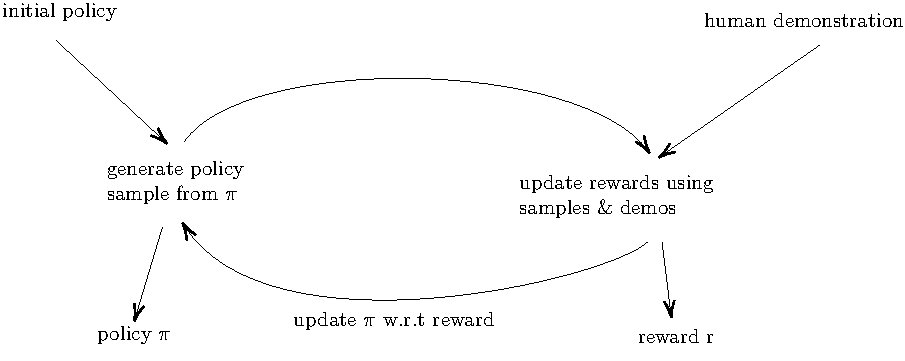
\includegraphics[width=0.7\linewidth]{content/tikz/guided_cost.pdf}
    \end{center}
\end{frame}

\begin{frame}
    \frametitle{IRL and GANs}

    \begin{itemize}
        \item Policy tries to fool the reward that it is a human demo
        \item Reward tries to distinguish between human demo and artificial one
    \end{itemize}

    Correspondence:

    \begin{columns}[c] % The "c" option specifies centered vertical alignment while the "t" option is used for top vertical alignment
        \begin{column}{0.5\textwidth} % Right column width
            \begin{itemize}
                \item trajectory $\tau$
                \item policy $\pi \thicksim q(\tau)$
                \item reward $\mathbf{r}$
            \end{itemize}
        \end{column}
        \begin{column}{0.5\textwidth} % Left column width
            \begin{itemize}
                \item sample $\mathbf{x}$
                \item generator $\mathbf{G}$
                \item discriminator $\mathbf{D}$
            \end{itemize}
        \end{column}
    \end{columns}


\end{frame}

\section{Review of latest works}

\begin{frame}
    \frametitle{OPIRL: Sample Efficient Off-Policy Inverse Reinforcement Learning via Distribution Matching \cite{hoshino_opirl_2022}}

    \begin{center}
        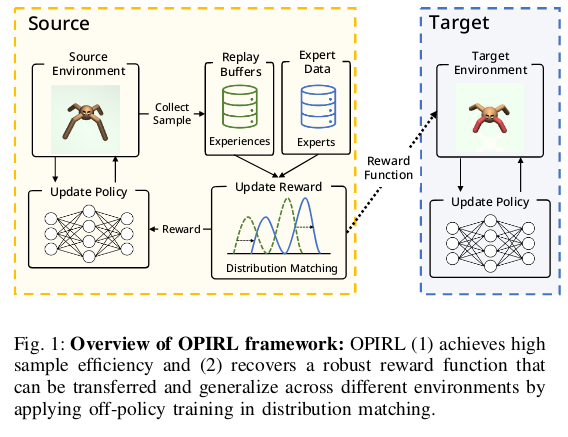
\includegraphics[width=0.4\linewidth]{content/images/oripl/im1.png}
    \end{center}
\end{frame}

\begin{frame}
    \frametitle{OPIRL: Sample Efficient Off-Policy Inverse Reinforcement Learning via Distribution Matching \cite{hoshino_opirl_2022}}

    \begin{center}
        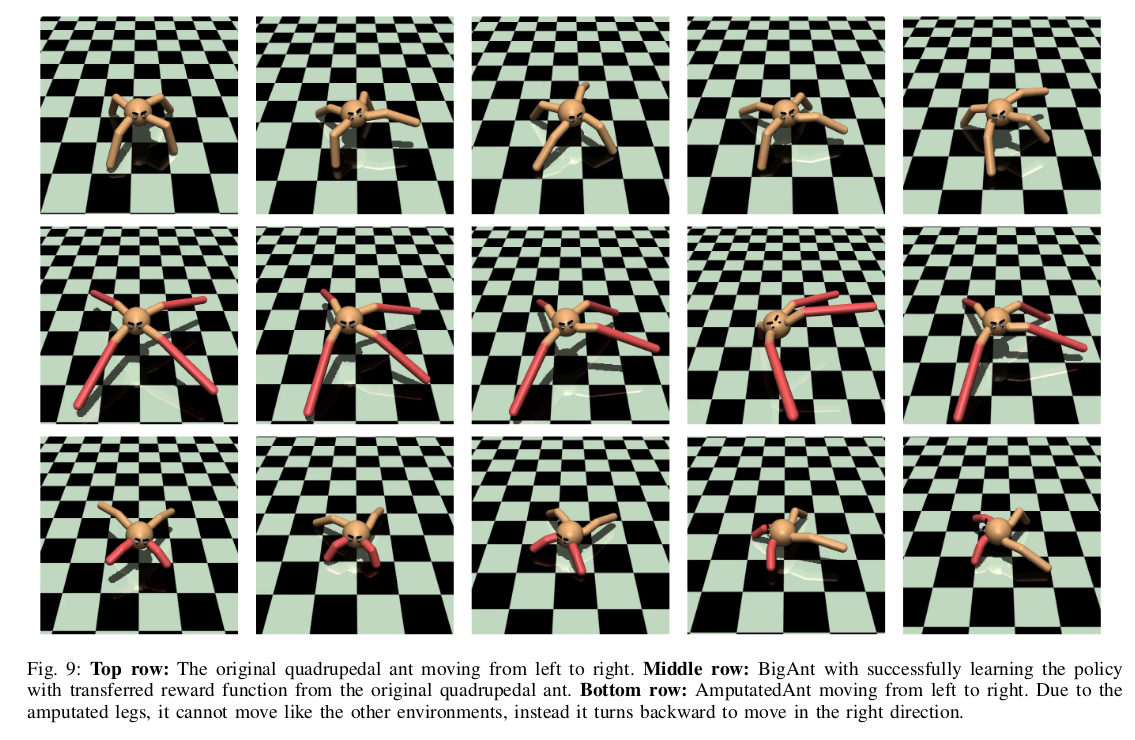
\includegraphics[width=0.55\linewidth]{content/images/oripl/im2.png}
    \end{center}
\end{frame}

\begin{frame}
    \frametitle{{DriveIRL}: {Drive} in {Real} {Life} with {Inverse} {Reinforcement} {Learning} \cite{phan-minh_driveirl_2023}}

    \begin{center}
        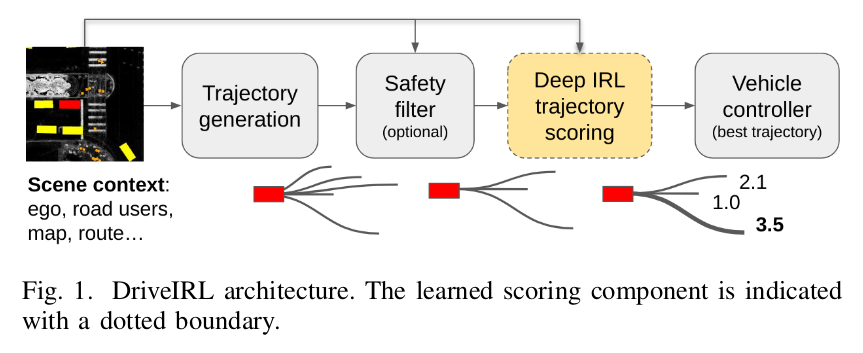
\includegraphics[width=0.55\linewidth]{content/images/driveirl.png}
    \end{center}
\end{frame}

\begin{frame}
    \frametitle{Human-{Guided} {Motion} {Planning} in {Partially} {Observable} {Environments} \cite{quintero-pena_human-guided_2022}}

    \begin{center}
        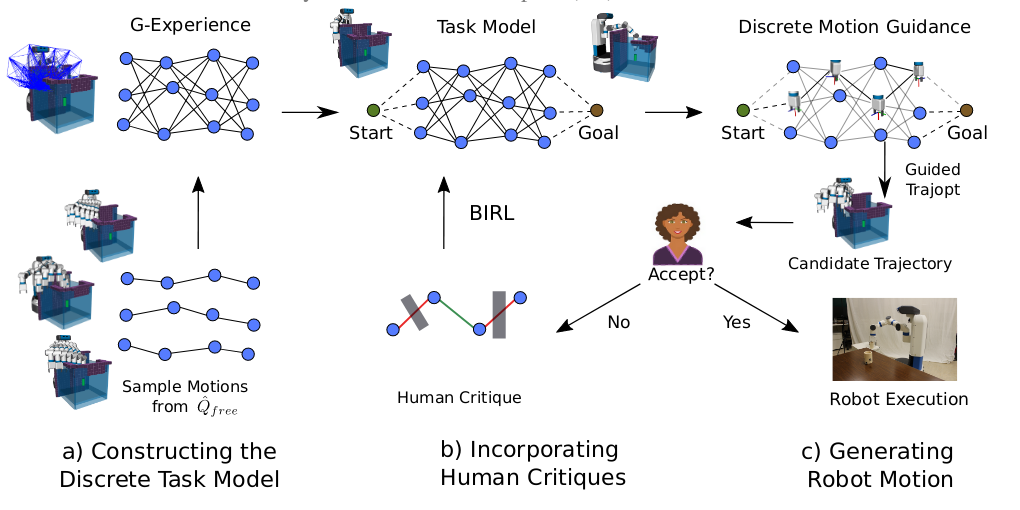
\includegraphics[width=0.55\linewidth]{content/images/human_guided.png}
    \end{center}
\end{frame}

\begin{frame}
    \frametitle{Inverse {Reinforcement} {Learning} {Framework} for {Transferring} {Task} {Sequencing} {Policies} from {Humans} to {Robots} in {Manufacturing} {Applications} \cite{manyar_inverse_2023}}

    \begin{center}
        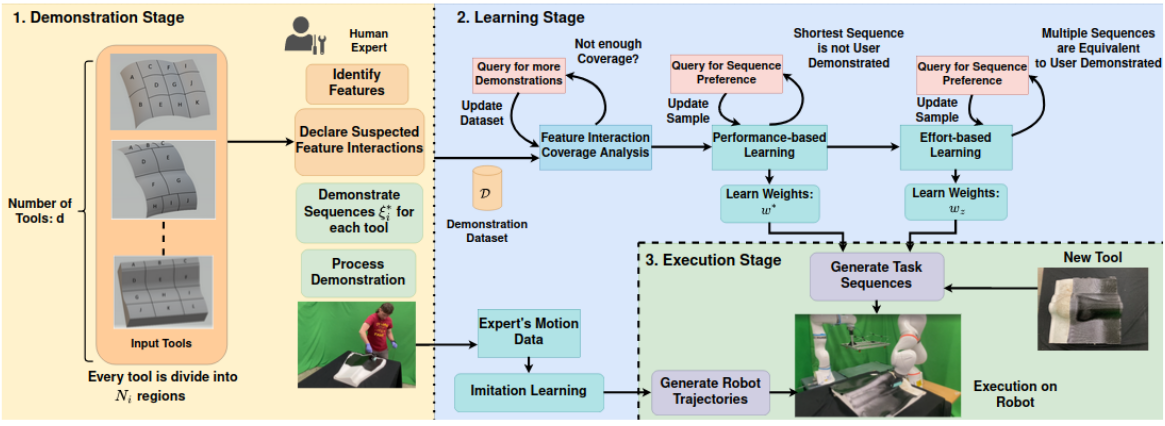
\includegraphics[width=0.7\linewidth]{content/images/inversereinforce.png}
    \end{center}
\end{frame}

\begin{frame}
    \frametitle{Online Prediction of Lane Change with a Hierarchical Learning-Based Approach \cite{liao_online_2022}}

    \begin{center}
        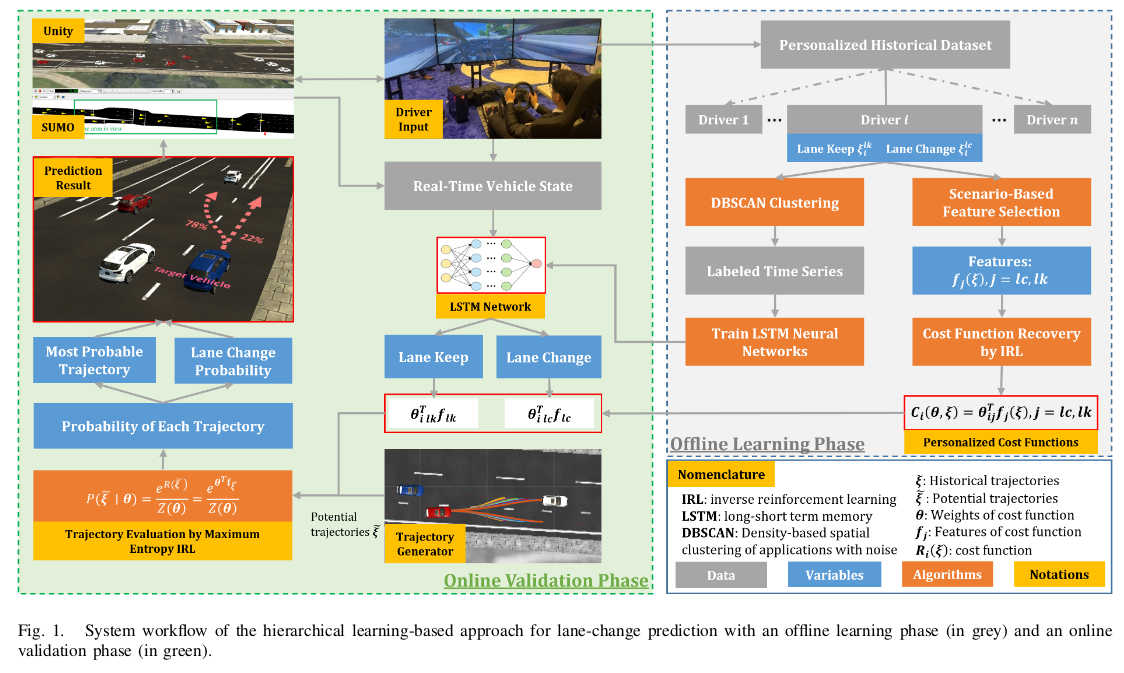
\includegraphics[width=0.6\linewidth]{content/images/lanechange.png}
    \end{center}
\end{frame}

\begin{frame}
    \frametitle{Personalized Car Following for Autonomous Driving with Inverse Reinforcement Learning \cite{zhao_personalized_2022}}

    \begin{center}
        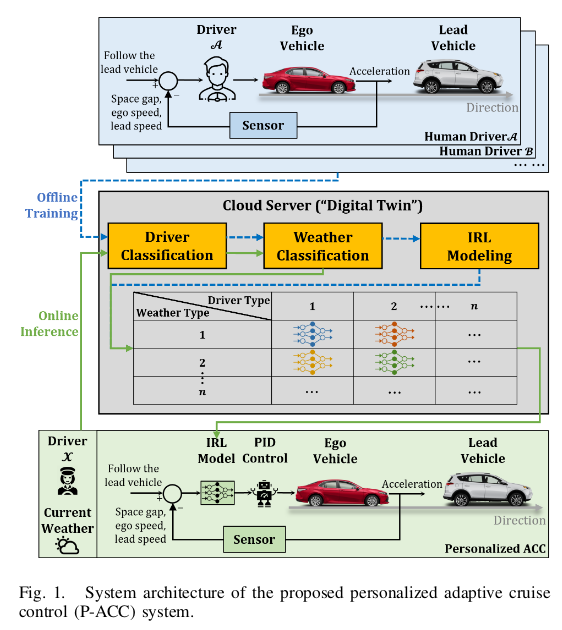
\includegraphics[width=0.35\linewidth]{content/images/personalized_car.png}
    \end{center}
\end{frame}

% \section{Motivation} % Note all sections and subsections are automatically placed in your table of contents

% %------------------------------------------------
% \begin{frame}
%     \frametitle{Title}
%     \begin{center}
%         \textbf{To use this template, you can copy and just edit/add slides!}\newline
%     \end{center}

%     This is because all of the color customization occurs in the "Customize Themes" section in lines 12-51 of the code\newline

%     The remainder of these slides serve as an example to show all the features you can use: bullets, buttons, sections, etc.

%     \begin{center}
%         \emph{This was a labor of love, I hope you like it!}
%     \end{center}
% \end{frame}

% %------------------------------------------------
% \begin{frame}
%     \frametitle{Another Title}
%     \framesubtitle{and a subtitle!}

%     Look at the code of this slide to see how columns made this formatting look nice.

%     % \begin{columns}[t] % The "c" option specifies centered vertical alignment while the "t" option is used for top vertical alignment
%     %     \begin{column}{0.5\textwidth} % Right column width
%     %         % To add an image %
%     %         \begin{figure}[h!]
%     %             \centering
%     %             %\caption{Hawkins et al, 2015}
%     %             \includegraphics[angle=0, width=4.5cm]{Hokie2.png}
%     %             %\label{Figure 1}
%     %         \end{figure}
%     %     \end{column}
%     %     \begin{column}{0.5\textwidth} % Left column width
%     %         \begin{figure}[h!]
%     %             \centering
%     %             %\caption{Hawkins et al, 2015}
%     %             \includegraphics[angle=0, width=4.5cm]{Hokie2.png}
%     %             %\label{Figure 1}
%     %         \end{figure}
%     %     \end{column}
%     % \end{columns}
% \end{frame}

% %------------------------------------------------
% \begin{frame}
%     \frametitle{Yet another title}
%     You can use bullets too:\newline
%     \begin{itemize}
%         \item Like this one\newline
%         \item \& this one
%     \end{itemize}
% \end{frame}

% %------------------------------------------------
% \begin{frame}
%     \label{Test} %For the link button for the Appendix slide
%     \frametitle{A title}

%     \begin{itemize}
%         \item You can also nest sub-bullets
%               \begin{itemize}
%                   \item Sub-bullet 1
%                   \item Sub-bullet 2
%                   \item Sub-bullet 3
%                   \item Sub-bullet 4 \newline
%               \end{itemize}
%     \end{itemize}

%     You can add citations \footcite{Tjøstheim} too\newline

%     \textbf{Below is a button that links to a slide in the appendix}

%     \begin{center}
%         \hyperlink{Figure}{\beamergotobutton{Go to graphs}}
%     \end{center}
% \end{frame}

% %------------------------------------------------
% \section{Theory}

% %------------------------------------------------
% \begin{frame}
%     \label{Test Stat}
%     \frametitle{The Test Statistic}

%     Here is a made up equation:
%     $$ \hat{A} = \bar{m}-\hat{m}_S$$ \newline

%     Notice how these buttons are centered and evenly spread out:\newline

%     \begin{columns}[t] % The "c" option specifies centered vertical alignment while the "t" option is used for top vertical alignment
%         \begin{column}{0.25\textwidth} % Right column width
%             \hyperlink{Terms}{\beamergotobutton{Go to Terms}}
%         \end{column}
%         \begin{column}{0.25\textwidth} % Left column width
%             \hyperlink{Definitions}{\beamergotobutton{Go to Definitions}}
%         \end{column}
%         \begin{column}{0.25\textwidth} % Left column width
%             \hyperlink{Theorems}{\beamergotobutton{Go to Theorems}}
%         \end{column}
%     \end{columns}

% \end{frame}

% %------------------------------------------------
% \begin{frame}
%     \frametitle{No way, another title!}
%     \begin{enumerate}
%         \item Instead of bullets, you can index by number too\newline
%         \item like this
%     \end{enumerate}
% \end{frame}

% %------------------------------------------------
% \section{Testing}

% %------------------------------------------------
% \begin{frame}
%     \frametitle{Second to last title}
%     \begin{block}{Block Title}
%         Block 1
%     \end{block}

%     \begin{exampleblock}{Example Block Title}
%         Block 2
%     \end{exampleblock}

%     \begin{alertblock}{Alert Block Title}
%         Block 3
%     \end{alertblock}

%     \begin{block}{} % Block without title
%         Block without a title
%     \end{block}
% \end{frame}

% %------------------------------------------------
% \section{Conclusion}
% %------------------------------------------------
% \begin{frame}
%     \frametitle{Last title}

%     Last bit of text

% \end{frame}

%---------------------------------------------------------
%	CLOSING SLIDE
%---------------------------------------------------------

% To remove miniframe from top
% \appendix
% \setbeamertemplate{headline}{}
% \addtobeamertemplate{frametitle}{\vspace*{-\headheight}}{}

% \begin{frame}[noframenumbering] %So the end and appendix slides don't contribute to the page count
%     %[plain] % The optional argument 'plain' hides the headline and footline
%     %\frametitle{Questions?}

%     \begin{center}
%         {\LARGE Questions?}
%     \end{center}

% \end{frame}

%---------------------------------------------------------
%	REFERENCES
%---------------------------------------------------------

\begin{frame}[noframenumbering, allowframebreaks]
    \frametitle{References}
    \printbibliography
\end{frame}

% %------------------------------------------------
% \begin{frame}[noframenumbering]
%     \label{Figure}
%     \frametitle{Appendix - A figure}
%     \hyperlink{Test}{\beamerreturnbutton{Return to presentation}}

%     % \begin{figure}[h!]
%     %     \centering
%     %     %\caption{}
%     %     \includegraphics[angle=0, width=5cm]{Newey et al Graph.png}
%     %     %\label{fig}
%     % \end{figure}
% \end{frame}

% %------------------------------------------------
% \begin{frame}[noframenumbering]
%     \label{Terms}
%     \frametitle{Appendix - Terms}

%     \begin{columns}[t] % The "c" option specifies centered vertical alignment while the "t" option is used for top vertical alignment
%         \begin{column}{0.5\textwidth} % Right column width
%             Some Estimators:
%             \begin{itemize}
%                 \item Drift: $\hat{\delta}$
%                 \item Boundary: $\hat{b}(t)$
%             \end{itemize}
%         \end{column}
%         \begin{column}{0.5\textwidth} % Left column width
%             Some Variables:
%             \begin{itemize}
%                 \item $\hat{V}$
%                 \item $\hat{m}_S$
%                 \item $\bar{m}$
%                 \item $m_J(\tau)$\newline\newline
%             \end{itemize}
%         \end{column}
%     \end{columns}
%     \hyperlink{Test Stat}{\beamerreturnbutton{Return to presentation}}
% \end{frame}

% %------------------------------------------------
% \begin{frame}[noframenumbering]
%     \label{Definitions}
%     \frametitle{Appendix - Definitions}
%     \begin{enumerate}
%         \item A definition \newline
%     \end{enumerate}

%     \hyperlink{Test Stat}{\beamerreturnbutton{Return to presentation}}
% \end{frame}

% %------------------------------------------------
% \begin{frame}[noframenumbering]
%     \label{Theorems}
%     \frametitle{Appendix - Theorems}
%     \begin{enumerate}
%         \item A theorem\newline
%     \end{enumerate}

%     \hyperlink{Test Stat}{\beamerreturnbutton{Return to presentation}}
% \end{frame}

\end{document}